\documentclass[12pt]{article}
\linespread{1.3}
\usepackage{hyperref}
\usepackage{enumitem}
%\usepackage{enumerate}
\usepackage{changepage,lipsum,titlesec, longtable}
\usepackage{cite}
\usepackage{comment, xcolor}
\usepackage[pdftex]{graphicx}
  \graphicspath{{images/}, {images/stat/}}
  \DeclareGraphicsExtensions{.pdf,.jpeg,.png, .jpg}
\usepackage[cmex10]{amsmath}
\usepackage{tikz}
\usepackage{array} 
\usepackage{caption}
\usepackage{subcaption}
%\usepackage{subfigure} 
\newcommand{\grey}[1]{\textcolor{black!30}{#1}}
\newcommand{\red}[1]{\textcolor{red!50}{#1}}
\newcommand{\question}[1]{\textcolor{magenta}{\textbf{Question: } {#1}}}
\newcommand{\fref}[1]{Figure~\ref{#1}}
\newcommand{\tref}[1]{Table~\ref{#1}}
\newcommand{\eref}[1]{Equation~\ref{#1}}
\newcommand{\cref}[1]{Chapter~\ref{#1}}
\newcommand{\sref}[1]{Section~\ref{#1}}
\newcommand{\aref}[1]{Appendix~\ref{#1}}
\newcommand{\note}[0]{\textbf{Note: }}

\renewcommand{\labelenumii}{\theenumii}
\renewcommand{\theenumii}{\theenumi.\\arabic{enumii}.}

\oddsidemargin0cm
\topmargin-2cm %I recommend adding these three lines to increase the
\textwidth16.5cm %amount of usable space on the page (and save trees)
\textheight23.5cm

\makeatletter
\renewcommand\paragraph{\@startsection{paragraph}{4}{\z@}%
            {-2.5ex\@plus -1ex \@minus -.25ex}%
            {1.25ex \@plus .25ex}%
            {\normalfont\normalsize\bfseries}}
\makeatother
\setcounter{secnumdepth}{4} % how many sectioning levels to assign numbers to
\setcounter{tocdepth}{4}    % how many sectioning levels to show in ToC

% draw diagram
\usetikzlibrary{shapes.geometric, arrows}
\tikzstyle{data} = [font=\scriptsize, rectangle, rounded corners, minimum width=1.5cm, minimum height=1cm,align=left, draw=black, fill=black!30]
\tikzstyle{database} = [font=\scriptsize, rectangle, rounded corners, minimum width=3cm, minimum height=1cm,align=left, draw=black, fill=green!30]
\tikzstyle{query} = [font=\scriptsize,trapezium, trapezium left angle=70, trapezium right angle=110, minimum width=0.5cm, minimum height=0.5cm, text centered, draw=black, fill=blue!30]
\tikzstyle{process} = [font=\scriptsize,rectangle, minimum width=3cm, minimum height=1cm, text centered, draw=black, fill=orange!30]
\tikzstyle{spliter} = [font=\scriptsize,diamond, minimum width=2cm, minimum height=1cm, text centered, draw=black, fill=green!30]
\tikzstyle{decision} = [font=\scriptsize,diamond, minimum width=3cm, minimum height=1cm, text centered, draw=black, fill=green!30]
\tikzstyle{arrow} = [thick,->,>=stealth]
\tikzstyle{bi-arrow} = [thick,->,>=stealth]

\begin{document}
\title{Approach for calculating piece-wise regression line of energy vs. temperature\\
  \large GSA project}
\maketitle
\tableofcontents
\section{Introduction}
The document records a possible way to calculate the piece-wise
regression line for each building.

From the initial plots of the buildings, there seems to be a large
variation in the inflation point (see Appendix)

\subsection{Brute force}
\subsubsection{Natural Gas}
The shape of the curve should have a inflation point. When temperature
is below the temperature, the natural gas consumption increases
linearly with the decreasing of the temperature.

There are only 36 points in the analysis, which allows for a brute
force approach as follows:

\begin{verbatim}
The input point P = [(x1, y1), (x2, y2), ..., (xn, yn)], 
Sort the points in P by x axis: P_sorted = sorted(P, key = x value)
partition P_sorted into two sets of points: P_1 and P_2
P_1 contains the first m elements of P_sorted and P_2 contains the
rest
m can range from 2 to (n - 2)

erros = []
for each m in 2 to (n - 2):
    compute regression for P_1_m and get line L_1_m
    compute regression for P_1_m and get line L_2_m
    compute the intersection point of L_1_m and L_2_m, call it C_m
    compute the squared error of E_1_m = (P_1_m, L_1_m) and E_2_m = (P_2_m, L_2_m)
    E_m = E_1_m + E_2_m
    erros.append(E_m)

Find the least error e_i in erros, the corresponding i is the partition
index of the points and the corresponding intersection, C_i, is the 
inflation point, the y-axis of C_i is the base load
\end{verbatim}

\subsubsection{Electricity}
Break into two cases: one inflation point and two inflation points.
Calculate both case and take the best fit of the two cases
\begin{verbatim}
Case I: one inflation point. 
the computation process is the same as in natural gas.

Case II: two inflation point. 
partition P_sorted into two sets of points: P_1 and P_2
P_1 contains the first m elements of P_sorted and P_2 contains the
rest
m can range from 2 to (n - 2)
Partition P_1 into two sets of points: P_11 and P_12, P_11 contains the first n points of P_1 and P_12 contains the rest of P_1

erros = []
for m in [2, n - 2]:
    for n in [2, m - 2]:
        compute regression for P_11_mn and get line L_11_mn
        compute regression for P_12_mn and get line L_12_mn
            restrict the form of line L_12_mn to be y = b, b is some constant
        compute regression for P_2_mn and get line L_2_mn
        compute the intersection point of L_11_mn and L_12_mn, call it C1_mn
        compute the intersection point of L_12_mn and L_2_mn, call it C2_mn
        compute the squared error of E_11_mn = (P_11_mn, L_11_mn), 
                                     E_12_mn = (P_12_mn, L_12_mn),
                                 and E_2_mn = (P_2_mn, L_2_mn)
        E_mn = E_11_mn + E_12_mn + E_2_mn
        erros.append(E_mn)

Find the best fit E_mn in erros, the corresponding m, n decides the inflation points.
\end{verbatim}
\pagebreak
\section{Appendix}
\begin{figure}[h!]
  \centering
  \begin{subfigure}{.4\textwidth}
  \centering
  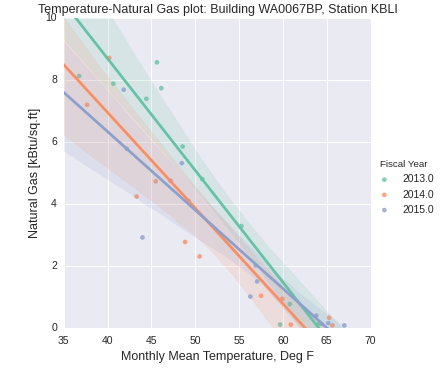
\includegraphics[width=\linewidth]{WA0067BP_KBLI_gas.png}
  \caption{Dot plot of monthly natural gas consumption vs. temperature}
  \label{fig:WA0067BP_KBLI_gas}
\end{subfigure}
%
\begin{subfigure}{.4\textwidth}
  \centering
  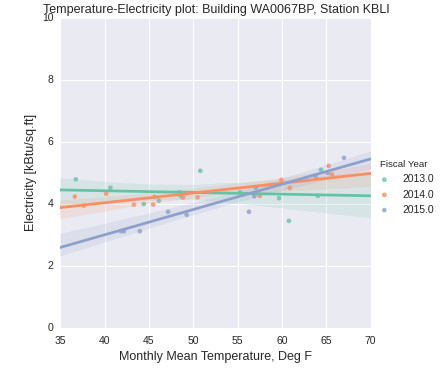
\includegraphics[width=\linewidth]{WA0067BP_KBLI_elec.png}
  \caption{Dot plot of monthly natural electricity consumption vs. temperature}
  \label{fig:WA0067BP_KBLI_elec}
\end{subfigure}
\end{figure}

\begin{figure}[h!]
  \centering
  \begin{subfigure}{.4\textwidth}
  \centering
  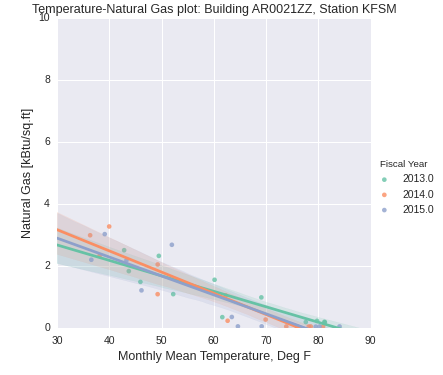
\includegraphics[width=\linewidth]{AR0021ZZ_KFSM_gas.png}
  \caption{Dot plot of monthly natural gas consumption vs. temperature}
  \label{fig:AR0021ZZ_KFSM_gas}
\end{subfigure}
%
\begin{subfigure}{.4\textwidth}
  \centering
  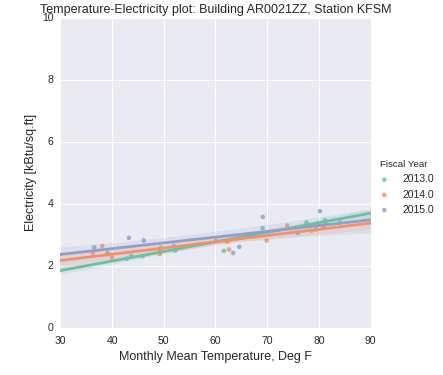
\includegraphics[width=\linewidth]{AR0021ZZ_KFSM_elec.png}
  \caption{Dot plot of monthly natural electricity consumption vs. temperature}
  \label{fig:AR0021ZZ_KFSM_elec}
\end{subfigure}
\end{figure}

\begin{figure}[h!]
  \centering
  \begin{subfigure}{.4\textwidth}
  \centering
  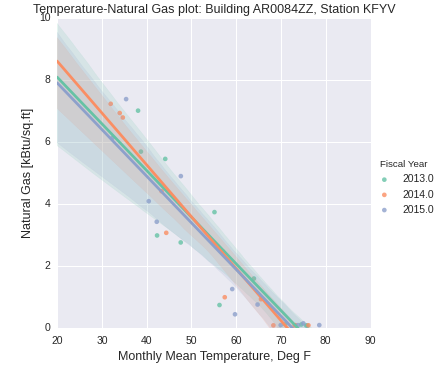
\includegraphics[width=\linewidth]{AR0084ZZ_KFYV_gas.png}
  \caption{Dot plot of monthly natural gas consumption vs. temperature}
  \label{fig:AR0084ZZ_KFYV_gas}
\end{subfigure}
%
\begin{subfigure}{.4\textwidth}
  \centering
  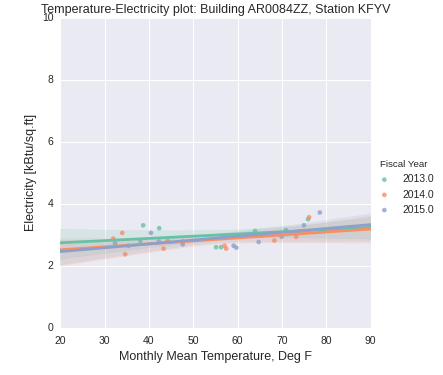
\includegraphics[width=\linewidth]{AR0084ZZ_KFYV_elec.png}
  \caption{Dot plot of monthly natural electricity consumption vs. temperature}
  \label{fig:AR0084ZZ_KFYV_elec}
\end{subfigure}
\end{figure}

\begin{figure}[h!]
  \centering
  \begin{subfigure}{.4\textwidth}
  \centering
  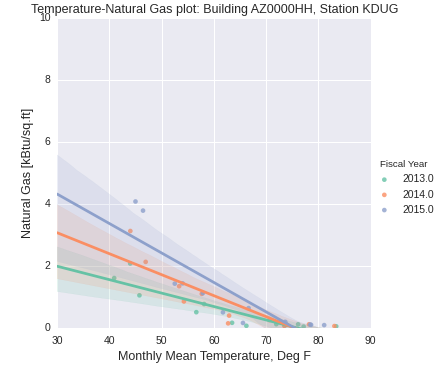
\includegraphics[width=\linewidth]{AZ0000HH_KDUG_gas.png}
  \caption{Dot plot of monthly natural gas consumption vs. temperature}
  \label{fig:AZ0000HH_KDUG_gas}
\end{subfigure}
%
\begin{subfigure}{.4\textwidth}
  \centering
  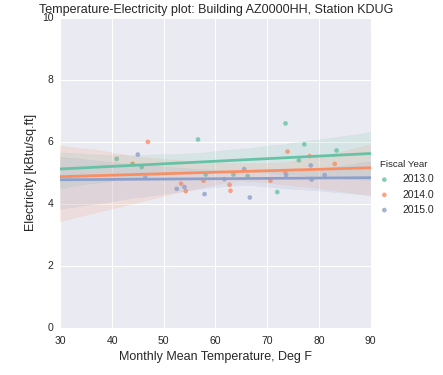
\includegraphics[width=\linewidth]{AZ0000HH_KDUG_elec.png}
  \caption{Dot plot of monthly natural electricity consumption vs. temperature}
  \label{fig:AZ0000HH_KDUG_elec}
\end{subfigure}
\end{figure}

\begin{figure}[h!]
  \centering
  \begin{subfigure}{.4\textwidth}
  \centering
  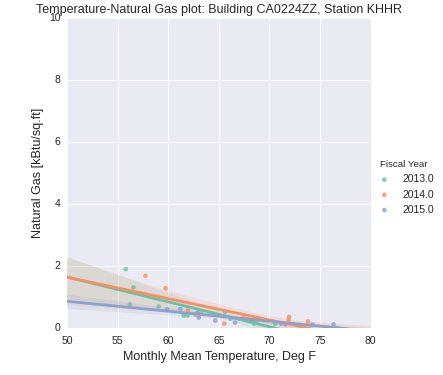
\includegraphics[width=\linewidth]{CA0224ZZ_KHHR_gas.png}
  \caption{Dot plot of monthly natural gas consumption vs. temperature}
  \label{fig:CA0224ZZ_KHHR_gas}
\end{subfigure}
%
\begin{subfigure}{.4\textwidth}
  \centering
  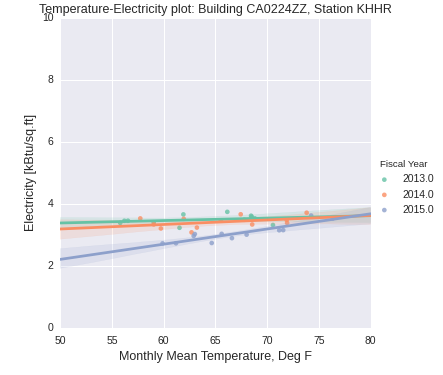
\includegraphics[width=\linewidth]{CA0224ZZ_KHHR_elec.png}
  \caption{Dot plot of monthly natural electricity consumption vs. temperature}
  \label{fig:CA0224ZZ_KHHR_elec}
\end{subfigure}
\end{figure}

\begin{figure}[h!]
  \centering
  \begin{subfigure}{.4\textwidth}
  \centering
  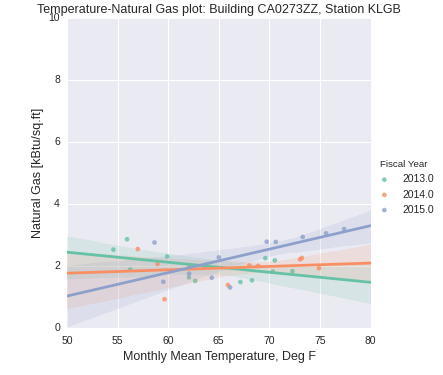
\includegraphics[width=\linewidth]{CA0273ZZ_KLGB_gas.png}
  \caption{Dot plot of monthly natural gas consumption vs. temperature}
  \label{fig:CA0273ZZ_KLGB_gas}
\end{subfigure}
%
\begin{subfigure}{.4\textwidth}
  \centering
  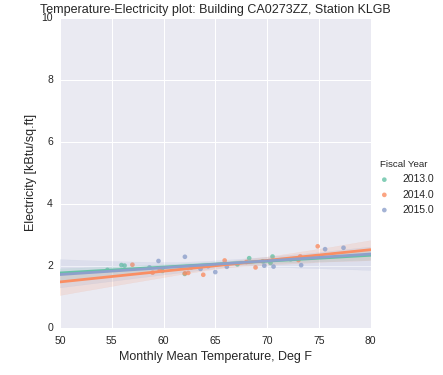
\includegraphics[width=\linewidth]{CA0273ZZ_KLGB_elec.png}
  \caption{Dot plot of monthly natural electricity consumption vs. temperature}
  \label{fig:CA0273ZZ_KLGB_elec}
\end{subfigure}
\end{figure}

\begin{figure}[h!]
  \centering
  \begin{subfigure}{.4\textwidth}
  \centering
  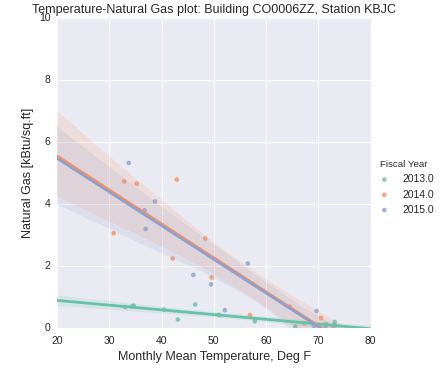
\includegraphics[width=\linewidth]{CO0006ZZ_KBJC_gas.png}
  \caption{Dot plot of monthly natural gas consumption vs. temperature}
  \label{fig:CO0006ZZ_KBJC_gas}
\end{subfigure}
%
\begin{subfigure}{.4\textwidth}
  \centering
  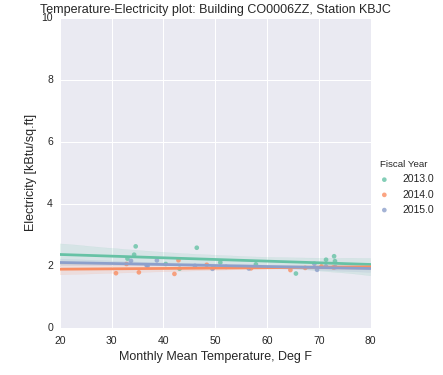
\includegraphics[width=\linewidth]{CO0006ZZ_KBJC_elec.png}
  \caption{Dot plot of monthly natural electricity consumption vs. temperature}
  \label{fig:CO0006ZZ_KBJC_elec}
\end{subfigure}
\end{figure}

\begin{figure}[h!]
  \centering
  \begin{subfigure}{.4\textwidth}
  \centering
  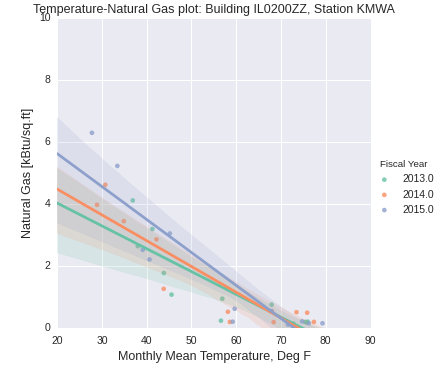
\includegraphics[width=\linewidth]{IL0200ZZ_KMWA_gas.png}
  \caption{Dot plot of monthly natural gas consumption vs. temperature}
  \label{fig:IL0200ZZ_KMWA_gas}
\end{subfigure}
%
\begin{subfigure}{.4\textwidth}
  \centering
  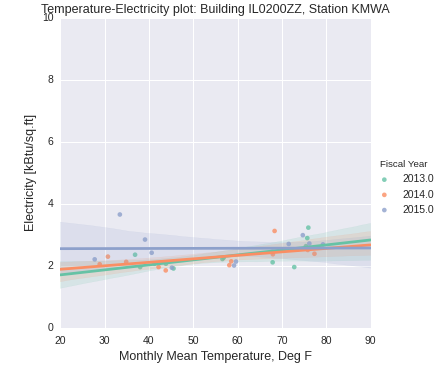
\includegraphics[width=\linewidth]{IL0200ZZ_KMWA_elec.png}
  \caption{Dot plot of monthly natural electricity consumption vs. temperature}
  \label{fig:IL0200ZZ_KMWA_elec}
\end{subfigure}
\end{figure}

\newpage
\bibliographystyle{plain} \bibliography{myCitation}
\end{document}